\chapter{Datasets}\label{chapter:dataset}
In this work, we use two different datasets to train and evaluate the performance of our framework. We use Microsoft Common Objects in Context (COCO) Dataset \cite{coco} for our 2D joints localization backbone and CMU Panoptic Dataset \cite{cmu-panoptic} for both the view-fusion and the temporal-fusion module.
\section{COCO 2017 Keypoint Dataset}
COCO is a large-scale object detection, segmentation, and captioning dataset. It is one of the best image datasets available, so it is widely used in cutting edge image recognition artificial intelligence research. It is used in open-source projects such as Facebook Research's Detectron. In our thesis, we use a subset of it from 2017 Keypoint Challenge, which contains masks, keypoint, and bounding boxes for the "person" class. See Fig. \ref{fig:ch5-coco-overview} for an overview of the most relevant part of the dataset to us
\begin{figure}
	\centering
	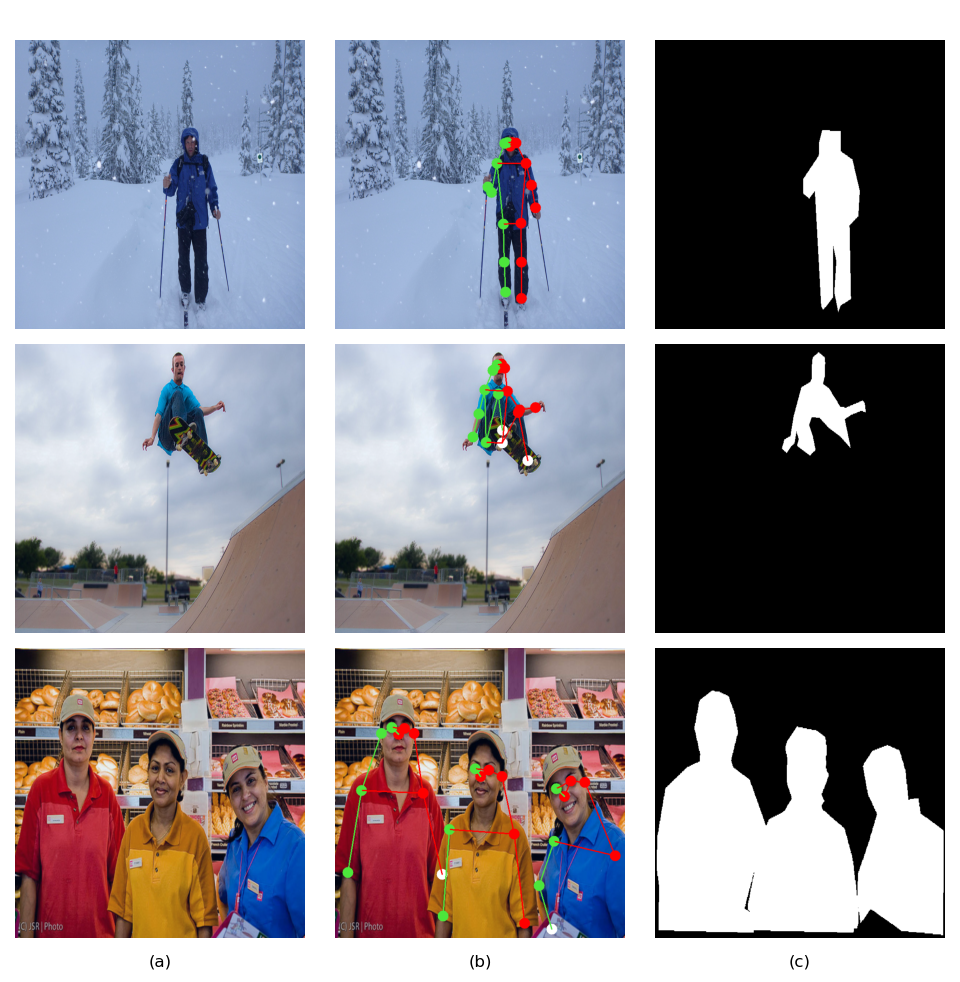
\includegraphics[width=1.0\columnwidth]{figures/ch5/coco-overview.png}
	\caption{Overview of 2017 COCO Keypoint. (a) Images with human (b) un-occluded (colored)/occluded (white) joint locations and limb (colored line), where green means left part of the body and red means right part of the body (c) masks for individuals} 
	\label{fig:ch5-coco-overview}
\end{figure}
\subsection{Annotation Format}
The COCO dataset is formatted in JSON and is a collection of “info”, “licenses”, “images”, “annotations”, “categories” (in most cases), and “segment info” (in one case).
\begin{lstlisting}[language=json,firstnumber=1, caption=Overview of JSON file in COCO 2017 Dataset]
{
"info": {...},
"licenses": [...],
"images": [...], 
"annotations": [...],
"categories": [...], <-- Not in Captions annotations,
"segment_info": [...] <-- Only in Panoptic annotations
}
\end{lstlisting}
We'll explain \textit{annotation} in detail, since we only use this for our work (in addition to the images).
\subsubsection{Person Annotation}
The annotation section contains a list of object with annotation infomation, see Listing \ref{lst:person-annotation}.
\begin{lstlisting}[language=json,firstnumber=1, caption=Overview of Person Class Annotation, label={lst:person-annotation}]
"annotations": [
{
"segmentation": [[204.01,306.23,...206.53,307.95]],
"num_keypoints": 15,
"area": 5463.6864,
"iscrowd": 0,
"keypoints": [229,256,2,...,223,369,2],
"image_id": 289343,
"bbox": [204.01,235.08,60.84,177.36],
"category_id": 1,
"id": 201376
}
]
\end{lstlisting}
The most important part for us are the iscrowd, segmentation, keypoints. We'll explain the meaning of the field:
\begin{description}
	\item [$\bullet$ segmentation], which are usually a list of polygon vertices around the object, but can also be a run-length-encoded (RLE) bit mask. Typically, RLE is used for groups of objects (like a large stack of books). We convert mask from a common polygon representation into a binary image $\mathbf{M}$ shown in Fig. \ref{fig:ch5-coco-overview} (c)
	
	\item [$\bullet$ iscrowd] specifies whether the segmentation is for a single object or a group/cluster of objects. In our work, we do not include images with "person" class and iscrowd with value 1.
	
	\item [$\bullet$ keypoints] are a list containing predefined 2D joint locations on the image of the \textit{i}-th individual. A list of keypoints has a length of 51, where every 3 elements can be grouped into a vector $\mathbf{x}_k^i \in \mathbb{R}^3$, specifically
	
	\begin{gather}
	\mathbf{x}_k^i = \left[x, y, v\right]^T, v = \left\{ 
	\begin{array}{ll}
	0\;, not\;annotated \\
	1\;, annotated\;but\;occluded\\
	2\;, annotated\;and\;visible\\
	\end{array}
	\right.
	\label{eq:joint-definition}
	\end{gather}
	, where \textit{not annotated} points have x and y set to 0. See Fig. \ref{fig:ch5-coco-overview} (b) for examples of $v = 1$ and $v=2$
	
	
\end{description}

\begin{table}[htpb]
	\caption[COCO keypoints and limb definition]{(left) COCO Keypoint and (right) limb definition.}\label{ch5:coco-definition}
	\centering
	\begin{tabular}{|c|c|c|}
		\toprule
		index & Joint Name & Definition\\
		\midrule
		1 & nose & - \\ \hline
		2 & eye\_l & left eye \\ \hline
		3 & eye\_r & right eye \\ \hline
		4 & ear\_l & left ear \\ \hline
		5 & ear\_r & right ear \\ \hline
		6 & sho\_l & left shoulder \\ \hline
		7 & sho\_r & right shoulder \\ \hline
		8 & elb\_l & left elbow \\ \hline
		9 & elb\_r & right elbow \\ \hline
		10 & wri\_l & left wrist \\ \hline
		11	 & wri\_r & right wrist \\ \hline
		12 & hip\_l & left hip \\ \hline
		13 & hip\_r & right hip \\ \hline
		14 & kne\_l & left knee \\ \hline
		15 & kne\_r & right knee \\ \hline
		16 & ank\_l & left ankle \\ \hline
		17 & ank\_r & right ankle \\
		\bottomrule
	\end{tabular}
	\hfill
	\begin{tabular}{|c|c| }
		\toprule
		index & limb\\
		\midrule
		1 & (ank\_l, kne\_left) \\ \hline
		2 & (kne\_l, hip\_l) \\ \hline
		3 & (ank\_r, kne\_r) \\ \hline
		4 & (kne\_r, hip\_r)  \\ \hline
		5 & (hip\_l, hip\_r) \\ \hline
		6 & (sho\_l, hip\_l) \\ \hline
		7 & (sho\_r, hip\_r)  \\ \hline
		8 & (sho\_l, sho\_r)  \\ \hline
		9 & (sho\_l, elb\_l)  \\ \hline
		10 & (sho\_r, elb\_r)  \\ \hline
		11 & (elb\_l, wri\_l)  \\ \hline
		12 & (elb\_r, wri\_r)  \\ \hline
		13 & (eye\_l, eye\_r)  \\ \hline
		14 & (nose, eye\_l)  \\ \hline
		15 & (nose, eye\_r)  \\ \hline
		16 & (eye\_l, ear\_l)  \\ \hline
		17 & (eye\_r, ear\_r)  \\ \hline
		18 & (ear\_l, sho\_l)  \\ \hline
		19 & (ear\_r, sho\_r)\\
		\bottomrule
	\end{tabular}	
\end{table}

\begin{figure}´
	\centering
	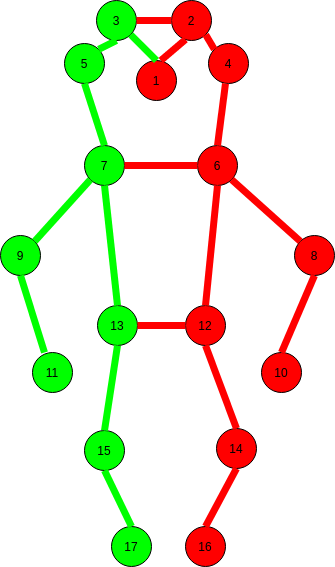
\includegraphics[width=0.3\columnwidth]{figures/ch5/coco-skeleton.png}
	\caption{COCO provide a reference skeleton (facing toward the reader) that connecting the joints. For our convenience in visualization, we define joints that belong to the left part of the body, colored with red, and to the right part of the body, colored with green.} 
	\label{fig:ch5-coco-skeleton}
\end{figure}

\begin{figure}
	\centering
	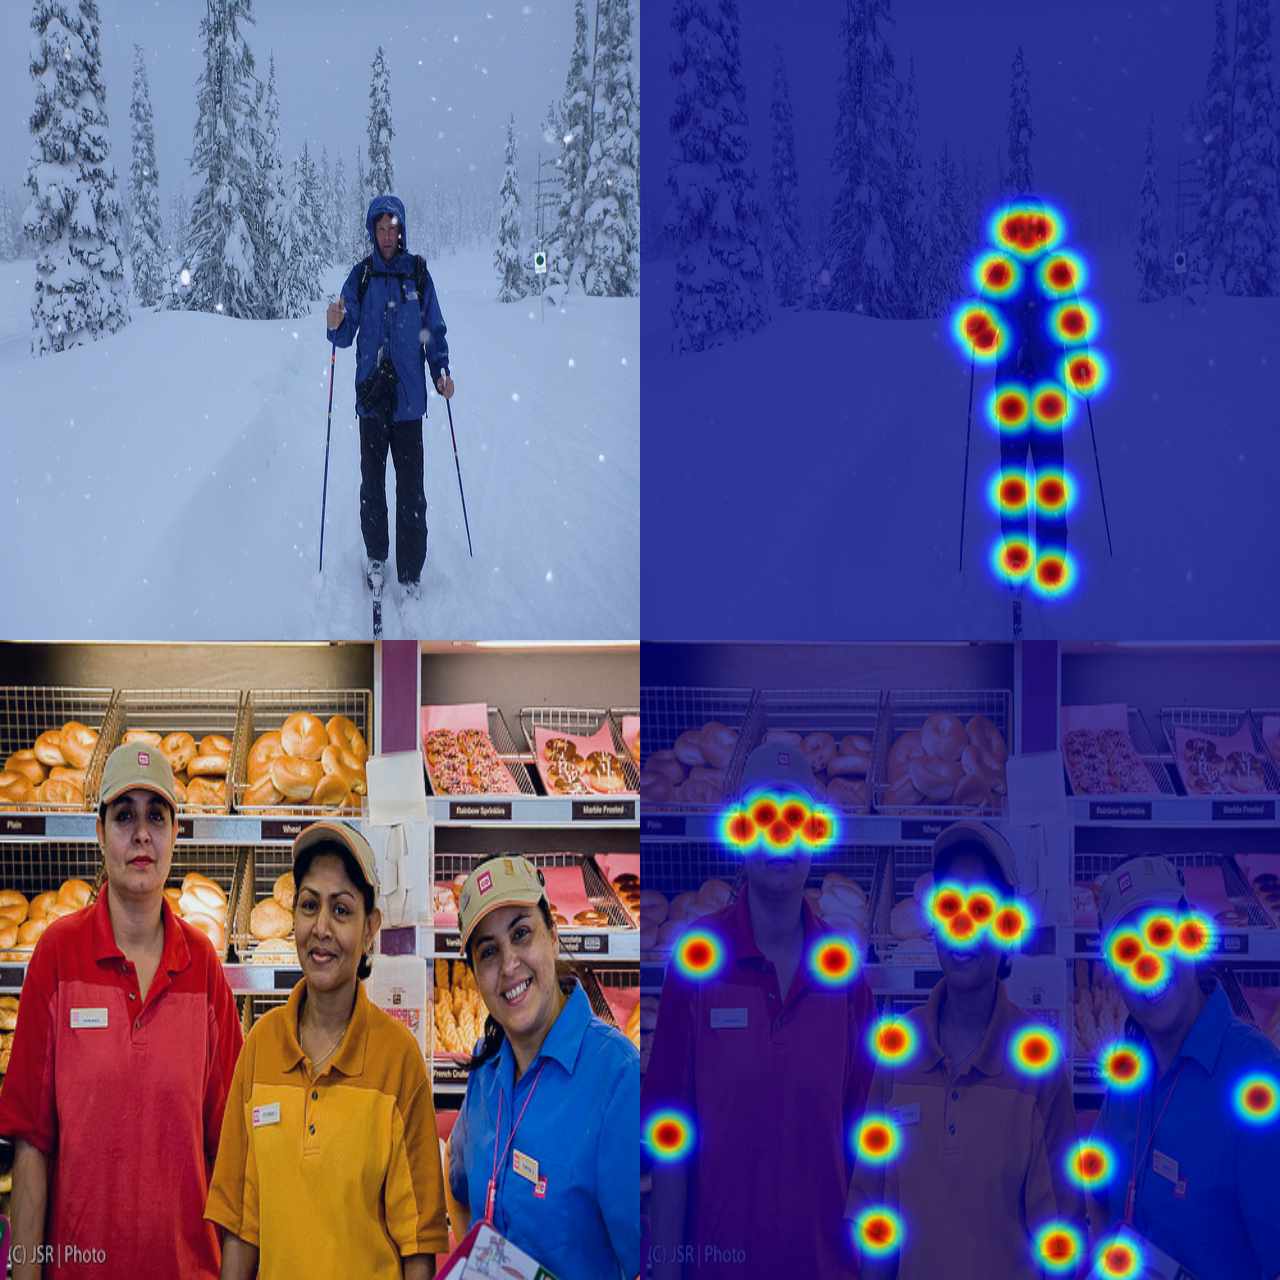
\includegraphics[width=0.5\columnwidth]{figures/ch5/coco-heatmap.png}
	\caption{(left column) The image with a person class label in COCO annotation and (right column) the joint heatmap $\mathbf{H}_k$. Note that, we merge all $K$ channels of joint heatmap to a single channel, in order to visuaulize compactly} 
	\label{fig:ch5-coco-heatmap}
\end{figure}

\subsection{Joint Heatmaps}
To estimate joint locations, we need a target that can feed into the CNN. Like many previous works, we use 2D heatmaps that indicating joint locations on images. For each joint $\mathbf{x}_k$, defined in Table. \ref{ch5:coco-definition}, we define a correspond heatmap $\mathbf{H}_k$, where $k$ denotes the k-th joint.

Recall that an individual's 2D joint $\mathbf{x}_k^i$ in (\ref{eq:joint-definition}) is defined as a 3-element vector with the first two elements indicating $x$ and $y$ coordinates, and the last element indicating visibility. The heatmap of an individual $\mathbf{H}_k^i$ is generated by placing a 2D Gaussian distribution at the joint location

\begin{gather}
\mathbf{H}_k^i(\mathbf{x}\mid\mathbf{x}_k^i) = 
\begin{cases}
\exp\left(-\frac{(x-x_k^i)^2 + (y-y_k^i)^2}{2\pi\sigma^2}\right),\ \text{if} & 
x_k^i - 3\sigma \leq x \leq x_k^i + 3\sigma \ \cap \\ 
& y_k^i - 3\sigma \leq y \leq y_k^i + 3\sigma \ \cap \\
& v_k^i > 0 \\
0, & \text{otherwise}
\end{cases}
\label{eq:joint-definition}
\end{gather}

Finally, a joint heatmap $\mathbf{H}_k$ that given $N$ individuals in an image is
\begin{gather}
\mathbf{H}_k(\mathbf{x}\mid(\mathbf{x}_k^1, \dots,  \mathbf{x}_k^N)) = 
\max \left(\mathbf{H}_k^1(\mathbf{x}\mid\mathbf{x}_k^1), \dots, \mathbf{H}_k^N(\mathbf{x}\mid\mathbf{x}_k^N)\right)
\label{eq:joint-heatmap}
\end{gather}
, shown in Fig. \ref{fig:ch5-coco-heatmap}.

\section{CMU Panoptic Dataset}
CMU Panoptic \cite{cmu-panoptic} is a dataset containing images with several people performing different scenarios (playing an instrument, dancing, etc.) in a dome
where several cameras are placed. The dataset provides synchronized videos from 480 VGA views and 31 HD views. All the sequences are annotated with estimated 3D joint locations and skeletons from using off-the-shelf 2D pose estimators and consensus voting method across view \cite{cmu-panoptic}. Even \textbf{without ground-truth annotations} of dataset, many state-of-art multi-person 3D pose researches \cite{voxelpose,Chen_2020_CVPR,20204DAssociation,iskakov2019learnable} are able to train and evaluate because of the large number of views.
\subsection{Annotation Format}
For each multi-view sequence, the dataset provides extrinsic matrices $\mathbf{K}$ and intrinsic matrices $\left[\mathbf{R}\mid \mathbf{t}\right]$ of both VGA and HD cameras. They also provide 3D joint locations $\mathbf{x}_{k_{3D}}^i$ for every individual with COCO-style annotation. One can project 3D joint location $\mathbf{x}_{k_{3D}}^i$ to 2D joint location $\mathbf{x}_{k}^i$, using the provided camera matrices with (\ref{eq:ch1-world-to-image-long}). However, the dataset does not provide any 2D annotation for occluded joints in a different view and, thus, one is not able to know if $\mathbf{x}_{k}^i$ being visible on the image or not, shown in Fig. \ref{fig:ch5-cmu-multiview}

\begin{lstlisting}[language=json,firstnumber=1, caption=Overview of Camera Annotation, label={lst:cmu-camera-matrix}]
{
"calibDataSource": "160223_calib_tent13_norm",
"cameras": [
{
"name": "01_01",
"type": "vga",
"resolution": [640,480],
"panel": 1,
"node": 1,
"K": [...],
"distCoef": [...],
"R": [...],
"t": [...]
}, ...
]
}
\end{lstlisting}

\begin{table}[htpb]
	\caption[COCO keypoints and limb definition]{(left) COCO Keypoint and (right) limb definition.}\label{ch5:coco-definition}
	\centering
	\begin{tabular}{|c|c|c|}
	\end{tabular}
\end{table}

\begin{figure}´
	\centering
	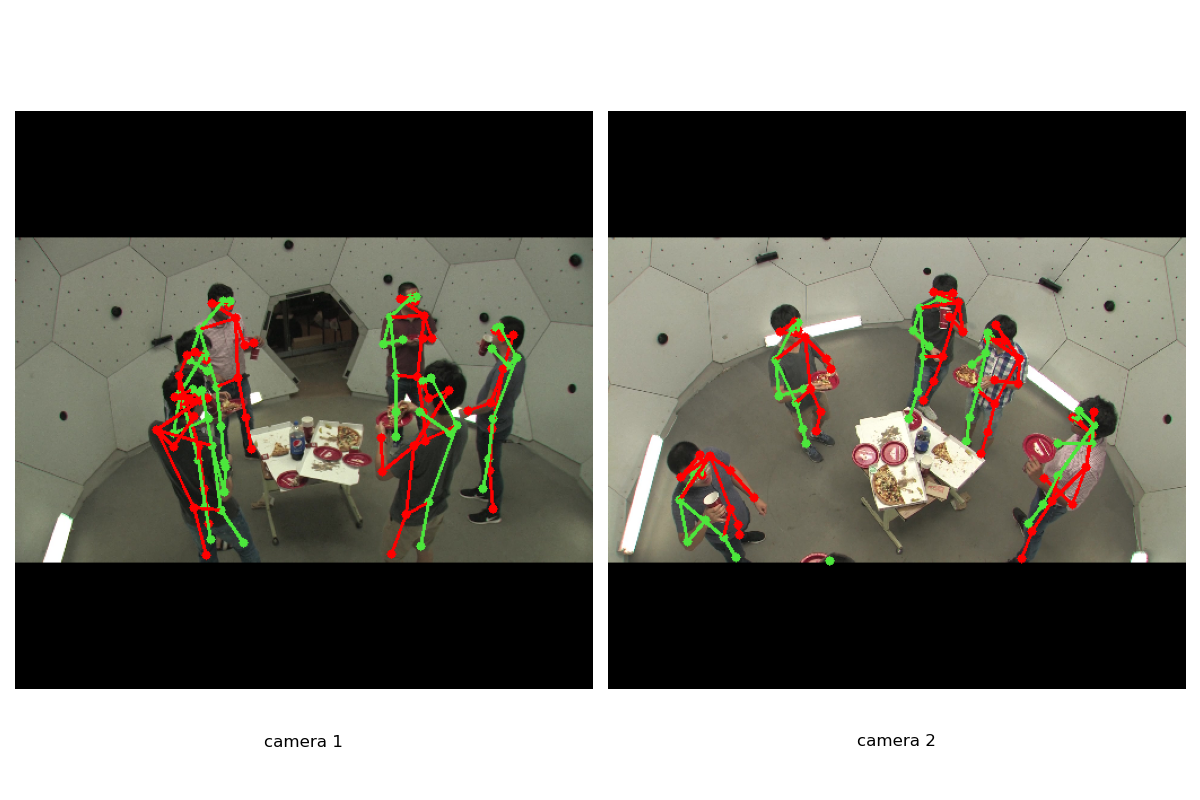
\includegraphics[width=0.7\columnwidth]{figures/ch5/panoptic-3d-annotation.png}
	\caption{CMU Panoptic Overview. Note that it does not provide 2D annotation about the visibility of projected 2D joints.} 
	\label{fig:ch5-cmu-multiview}
\end{figure}

\section{Data Augmentation}
Data augmentation has been a common practice in training deep neural network. In this work, we adopt image argumentation for COCO Dataset and augmentation on intrinsic camera matrices for CMU Panoptic Dataset.
\subsection{Image Augmentation}
A set of image augmentations are applied on both COCO, see Fig. \ref{fig:ch5-coco-augmentation}, and CMU Panoptic. For augmentating CMU dataset, we must update camera projection matrix $\mathbf{P}$ (\ref{eq:ch1-world-to-image-convention}) with an affine transformation parameterized by $\mathbf{A} \in \mathtt{R}^{2 \times 2}$ and $\mathbf{b} \in \mathtt{R}^2$.
\begin{gather}
\mathbf{P} \coloneqq 
\begin{bmatrix}
\mathbf{A} & \mathbf{b}\\
\mathbf{0^T} & 1
\end{bmatrix}
\mathbf{P}
\end{gather}
For example, scaling of a projection matrices, suppose the input image is spatially down-sampled $s_x$ and $s_y$ times along the x-axis and y-axis, the projection matrix $\mathbf{P}$ is updated as follows
\begin{gather}
\mathbf{P} \coloneqq 
\begin{bmatrix}
1/s_x & 0 & (1-s_x)/2s_x\\
0 & 1/s_y & (1-s_y)/2s_y\\
0 & 0 & 1\\
\end{bmatrix}
\mathbf{P}
\end{gather}
The coordinates are aligned with the center of pixels rather than the top-left corners. We can verify if we update the camera projection matrix correctly by observing the whether corresponding epiploar lines passing through the keypoint from the same person, see Fig. \ref{fig:ch5-cmu-epipolar-line}.

\begin{table}[htpb]
	\caption[Augmentations used in training]{Augmentations used in training.}\label{ch5:coco-definition}
	\centering
	\begin{tabular}{|c|c|c|c|c|}
		\toprule
		Dataset & rotation & translation & resizing & left-and-right flip \\ \hline
		COCO & $[-60, 60]$ & $[-50px,50px]$ & $[0.7\times, 1.3\times]$ & $50\%$ \\ \hline
		CMU Panoptic & $[-60, 60]$ & $[-50px,50px]$ & $[0.7\times, 1.3\times]$ & - \\ \hline
		\bottomrule
	\end{tabular}	
\end{table}

\begin{figure}´
	\centering
	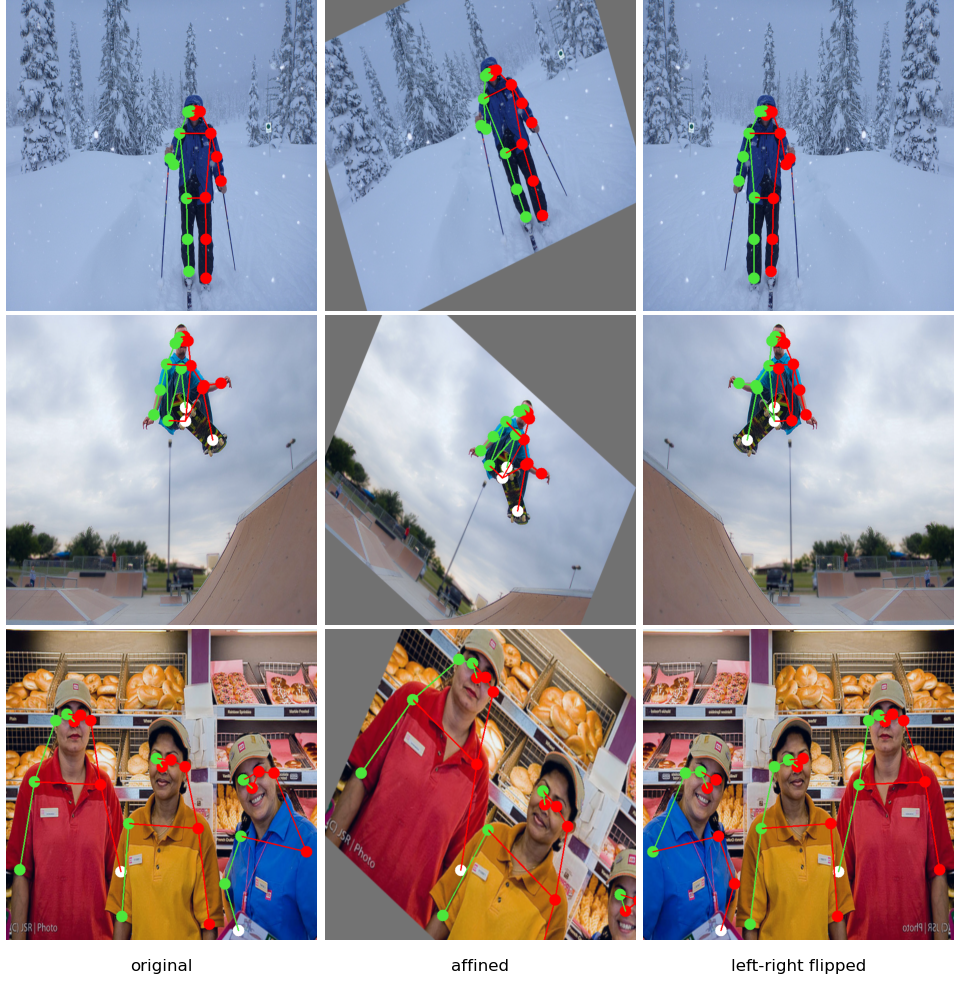
\includegraphics[width=0.7\columnwidth]{figures/ch5/coco-augmentation.png}
	\caption{Data augmentation for COCO Dataset} 
	\label{fig:ch5-coco-augmentation}
\end{figure}

\begin{figure}´
	\centering
	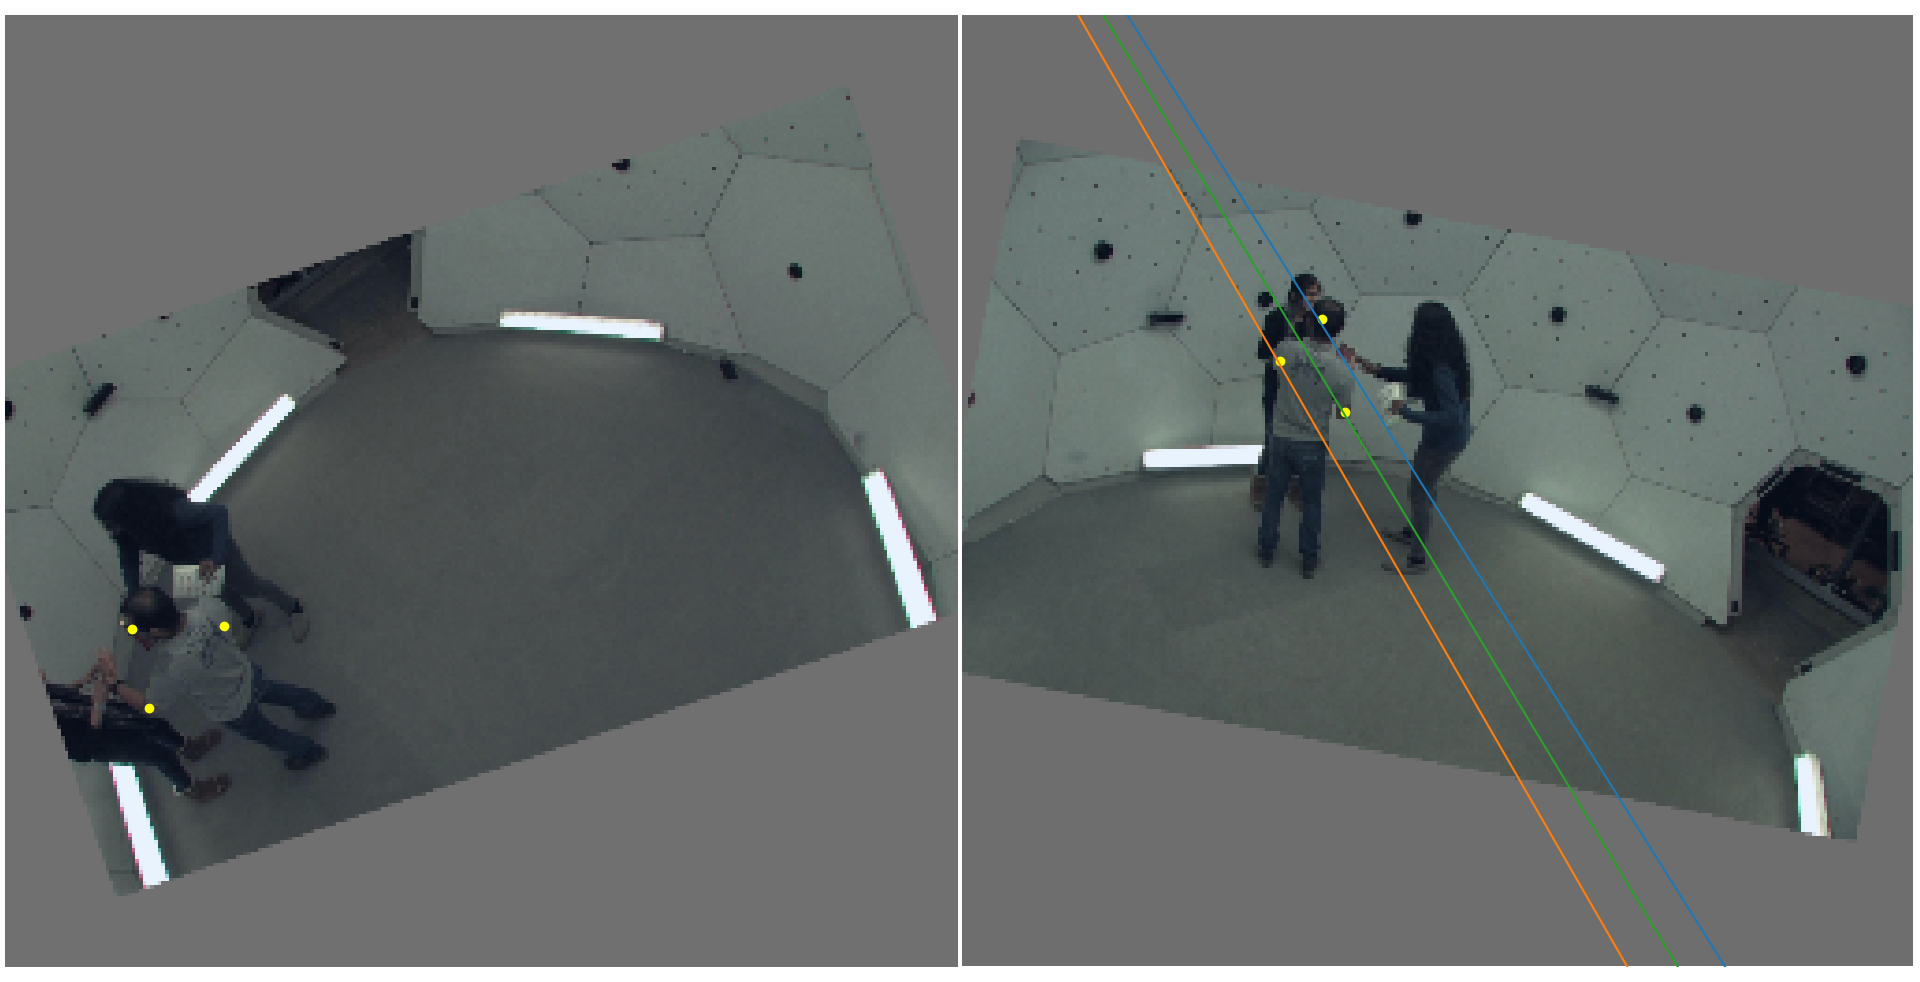
\includegraphics[width=1.0\columnwidth]{figures/ch5/panoptic-3d-epipolar-line.png}
	\caption{(left) keypoints from one view (right) correspond epiploar lines and the same keypoints in other view. Note that epiploar lines pass through the same keypoints in different views, verifying the camera projection matrix is updated correctly.} 
	\label{fig:ch5-cmu-epipolar-line}
\end{figure}

\subsection{Joint Augmentation}
We increased the total number of joints from 17 to 55, by interpolating two intermediate joints on each limb defined in \ref{ch5:coco-definition}. The intuition behind this is to use redundancy of joints to mitigate the effect of occlusion. These intermediate joints are placed at locations that are 0.1$\times$\textit{limb length} away from both ends of the limb.